\documentclass[12pt, onecolumn]{IEEEtran}
\usepackage[brazilian]{babel}
\usepackage[utf8]{inputenc}
\usepackage{amsmath}
\usepackage{mathtools}
\usepackage{indentfirst}
\usepackage{graphicx}
\usepackage{float}
\usepackage{booktabs}
\usepackage{siunitx}
\usepackage{tabularx}
\usepackage{caption}
\usepackage{subcaption}


\title{Relatório Experimental 3 - Prática de Física dos Dispositivos Eletrônicos}
\author{Felipe Rodrigues Sobrinho (17/0141764)}
\date{14/06/2022}


\begin{document}

\maketitle

\section{Introdução}

Os dispositivos transdutores são capazes de relacionar alguma grandeza física com
uma proporcional elétrica. Para a intensidade luminosa, é utilizado os resistores 
LDR ("\textit{Light Emmiter Dependent}"). Tais apresentam uma resistência muito alta
quando não está exposto a nenhuma luz, e decaí rapidamente para alguns ohms na presença
de alguma fonte luminosa.

Esse experimento então visa explorar essas características em dois passos distintos, 
os quais serão pós-processados para verificar se a experimentação condiz com os
modelos matemáticos que descrevem o comportamento do disposivo.

\section{Resultados}

\subsection{Questão 1}

Para esse experimento, foi utilizado uma fonte de tensão variável e um resistor em série com o LED, R2, no valor de $1k\Omega$, na disposição vista na figura \ref{fig:fig1}.

\begin{figure}[H]
  \centering
  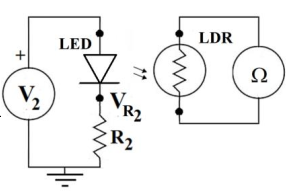
\includegraphics[width=.5\textwidth]{fig1}
  \caption{Esquemático do experimento.}
  \label{fig:fig1}
\end{figure}


Experimentalmente, foi obtido os seguintes dados vistos na tabela \ref{tab:q1}.


\begin{table}[H]
\centering
\caption{Resistência medida do LDR para diferentes Tensões sobre o resistor R2.}
\label{tab:q1}
\begin{tabular}{|c|c|c|c|l|l|l|l|}
\hline
$\mathbf{V_{R2 alvo}}$ & \textbf{0.0} & \textbf{0.5} & \textbf{1.0} & \textbf{1.5} & \textbf{2.0} & \textbf{2.5} & \textbf{3.0} \\ \hline
$\mathbf{V_{R2}}$      & $0V$            &$ 0.499V$        &$ 1.002V$        &$ 1.501V$        &$ 2.01V$         &$ 2.50V$         &$ 3.00V$         \\ \hline
$\mathbf{R_{LDR}}$     & $21.0 k\Omega$       & $1.115 k\Omega$      & $0.748 k\Omega$      & $0.601 k\Omega$      & $0.518 k\Omega$      & $0.464 k\Omega$        & $0.424 k\Omega$      \\ \hline
\end{tabular}
\end{table}

Com tais dados, é possível traçar uma curva da resistência do LDR em função 
da corrente aplicada no LED. Sabe-se que quanto mais corrente em um LED, 
maior a luminosidade, e consequentemente menor será a resistência do LDR, 
como pode ser visto na figura \ref{fig:q1_graph}.

\begin{figure}[H]
  \centering
  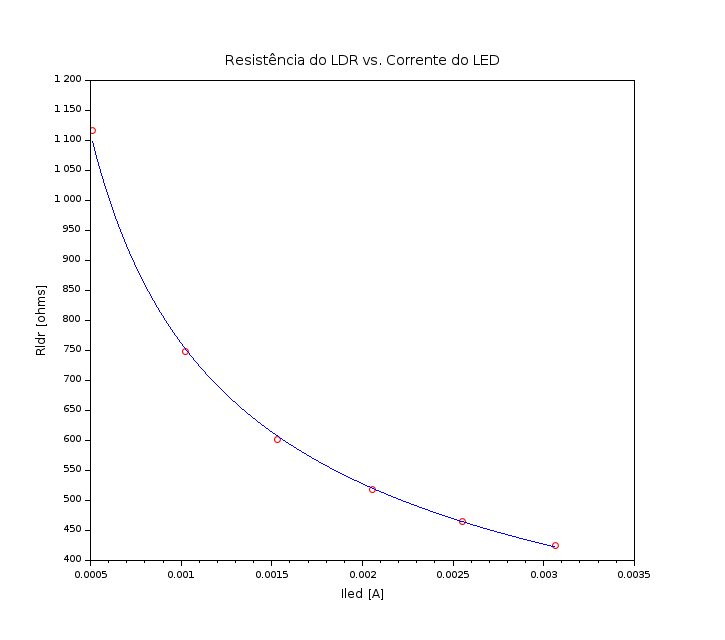
\includegraphics[width=.55\textwidth]{q1_graph}
  \caption{Gráfico da Resistência do LDR pela corrente no LED. Em azul, o modelo de ajuste aplicado.}
  \label{fig:q1_graph}
\end{figure}

Com o modelo de ajuste adotado visto na equação \ref{eq:q1}, podemos ajustar a
curva azul visto na figura \ref{fig:q1_graph}, que dá uma predição de qual será 
a resistência em relação a corrente. Com o erro quadrático médio percentual
de 0.0062272, pode-se dizer que o modelo adequou-se muito bem aos dados experimentais.


\begin{gather}\label{eq:q1}
  G_{LDR} = C_1\cdot \sqrt{2} + C2
\end{gather}


A figura \ref{fig:exp1_photos} mostra as medições feitas no experimento para a ratificação dos resultados.

\begin{figure}[H]
  \centering
  \begin{subfigure}{.3\textwidth}
    \centering
    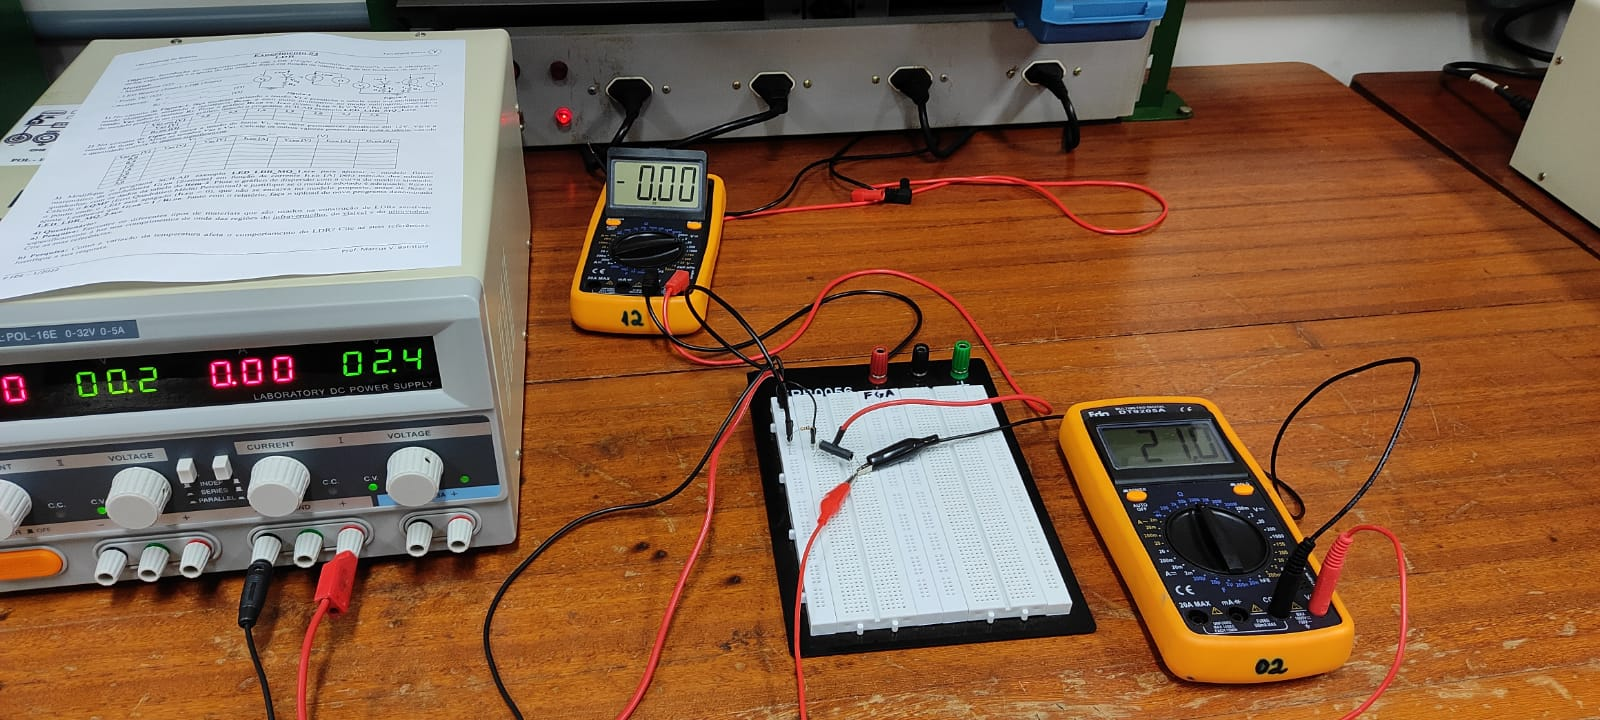
\includegraphics[width=\textwidth]{q1_0V}
    \caption{$V2_{alvo}=0V$}
  \end{subfigure}
  \begin{subfigure}{.3\textwidth}
    \centering
    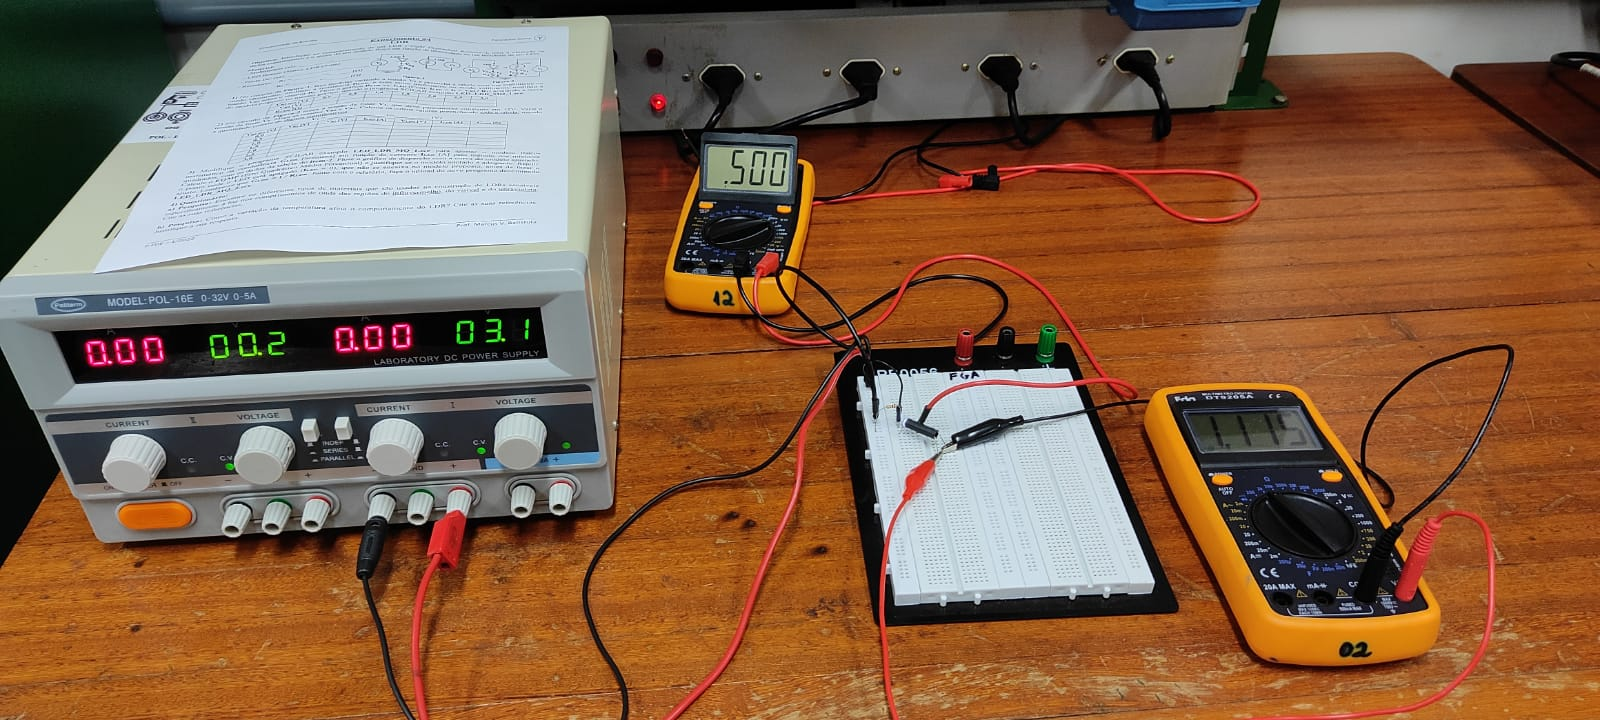
\includegraphics[width=\textwidth]{q1_0V5}
    \caption{$V2_{alvo}=0.5V$}
  \end{subfigure}
  \begin{subfigure}{.3\textwidth}
    \centering
    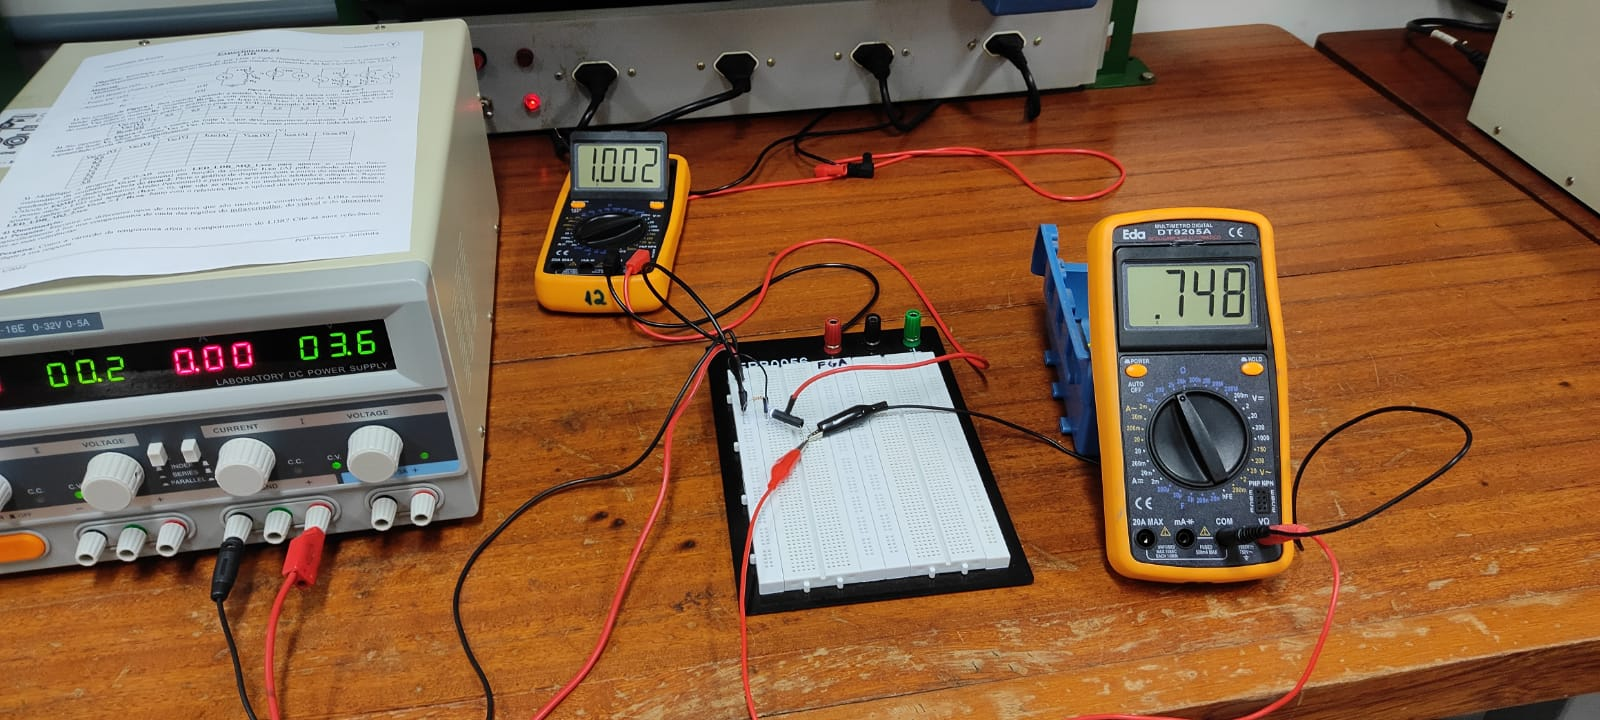
\includegraphics[width=\textwidth]{q1_1V}
    \caption{$V2_{alvo}=1V$}
  \end{subfigure}
  \begin{subfigure}{.3\textwidth}
    \centering
    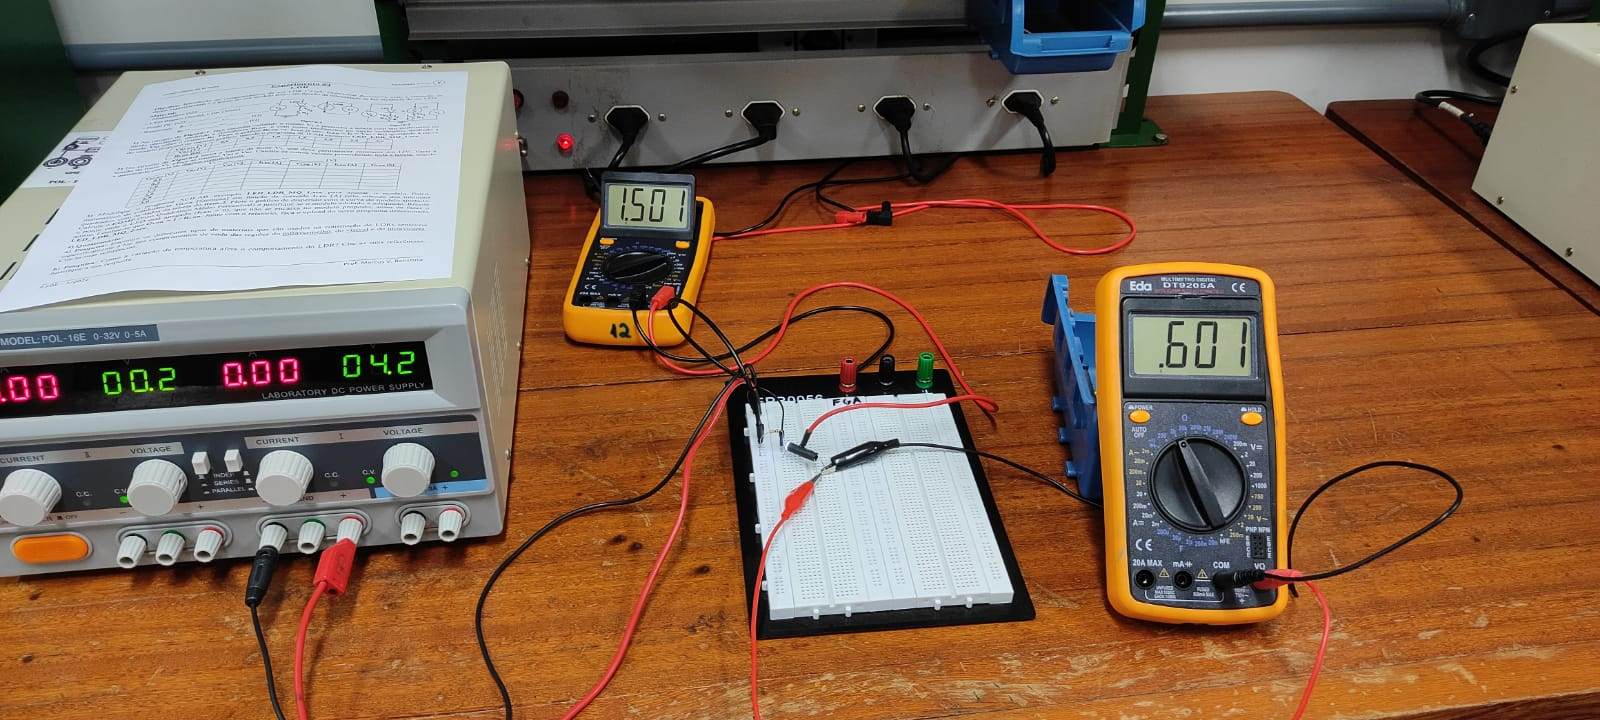
\includegraphics[width=\textwidth]{q1_1V5}
    \caption{$V2_{alvo}=1.5V$}
  \end{subfigure}
  \begin{subfigure}{.3\textwidth}
    \centering
    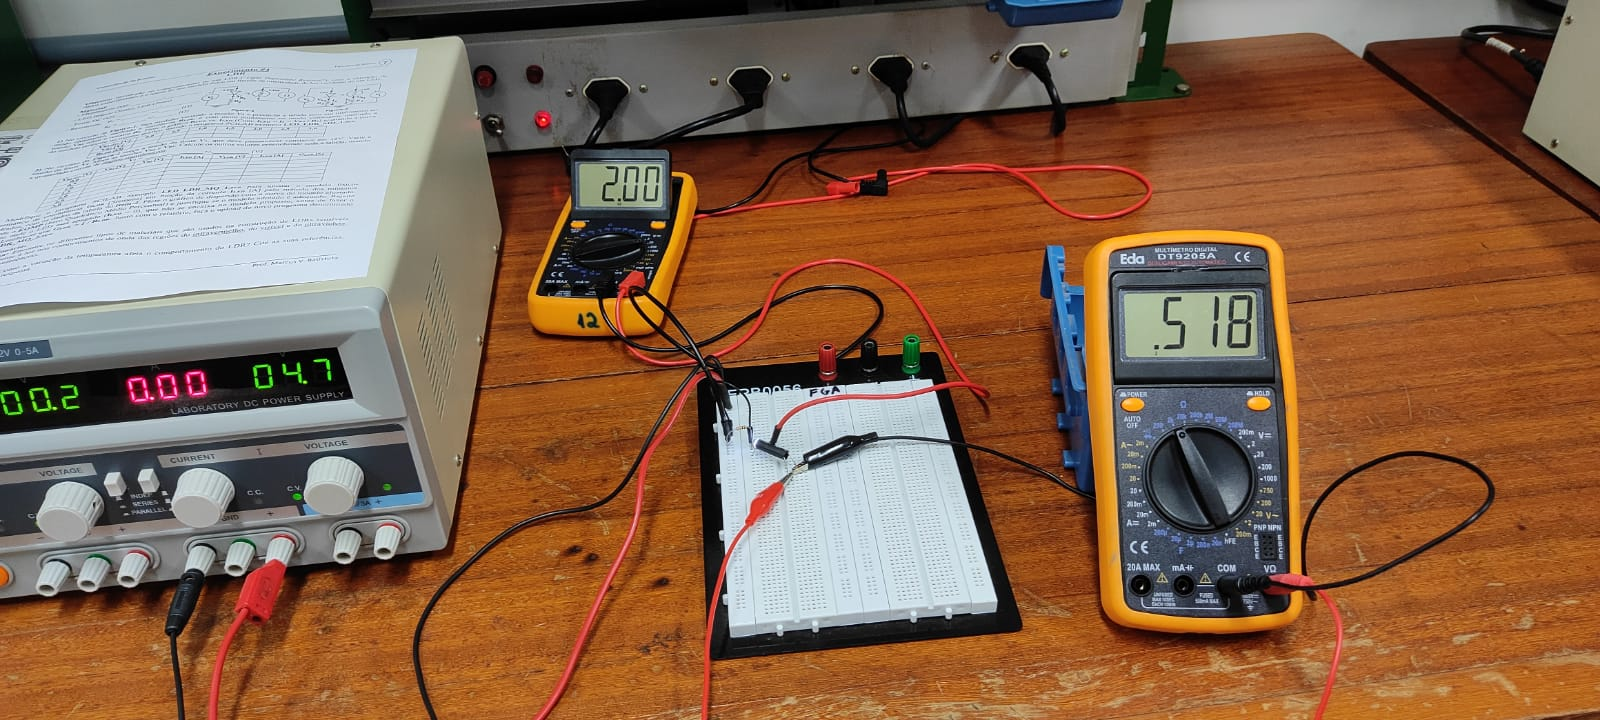
\includegraphics[width=\textwidth]{q1_2V}
    \caption{$V2_{alvo}=2V$}
  \end{subfigure}
  \begin{subfigure}{.3\textwidth}
    \centering
    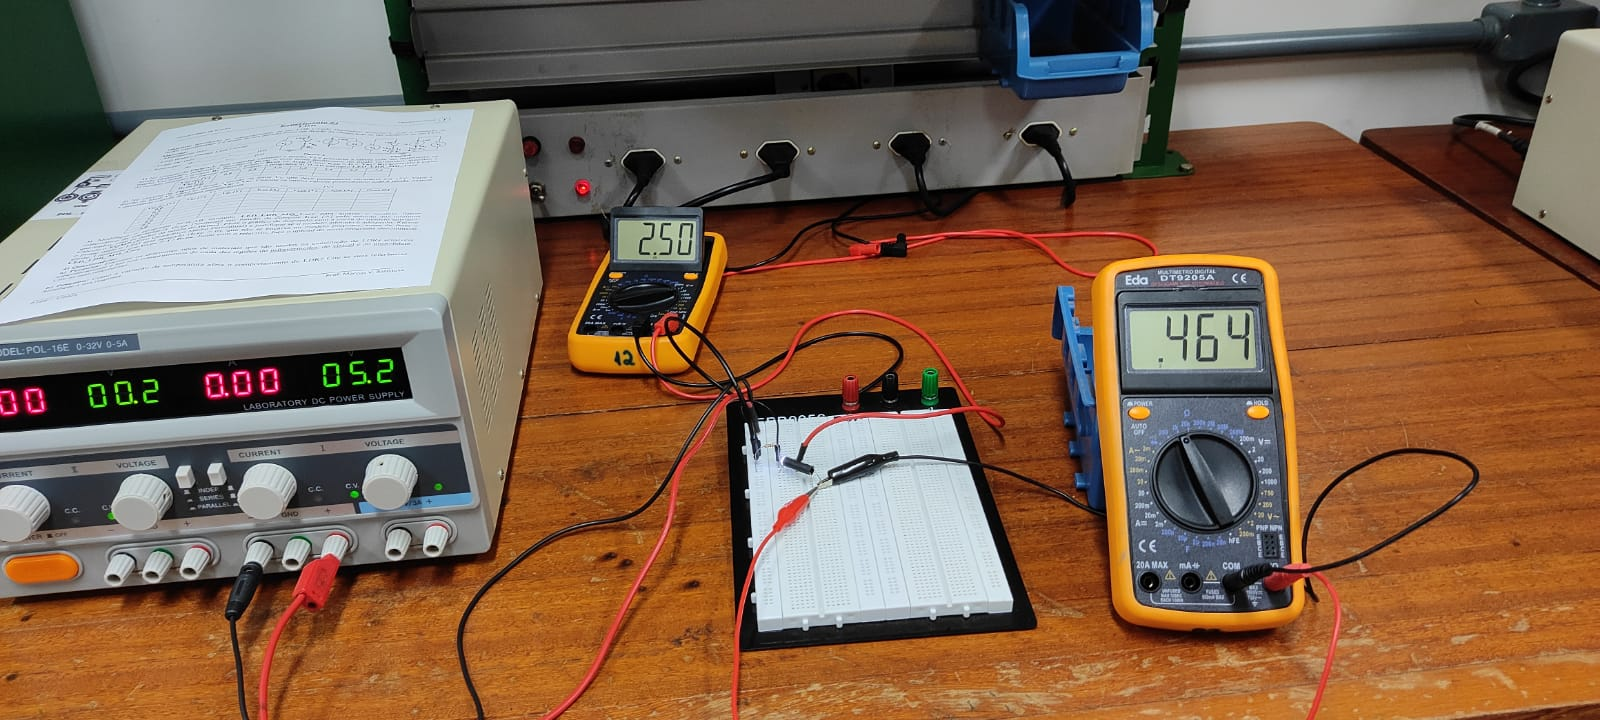
\includegraphics[width=\textwidth]{q1_2V5}
    \caption{$V2_{alvo}=2.5V$}
  \end{subfigure}
  \begin{subfigure}{.3\textwidth}
    \centering
    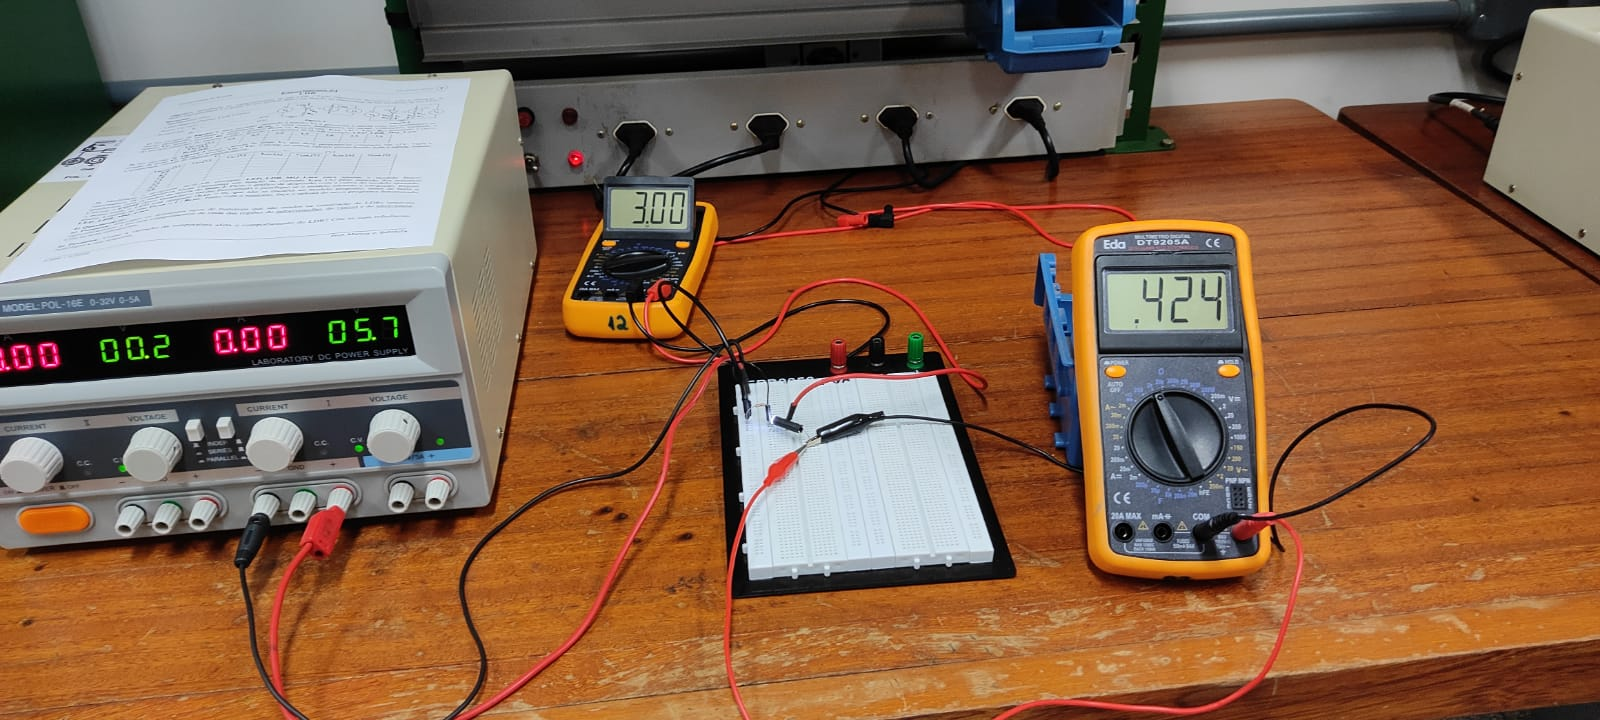
\includegraphics[width=\textwidth]{q1_3V}
    \caption{$V2_{alvo}=3V$}
  \end{subfigure}
  
  \caption{Medições realizadas para a primeira parte do experimento.}
  \label{fig:exp1_photos}
\end{figure}




\subsection{Questão 2}

Para tal experimento foi utilizado uma fonte de tensão variável (V1) e uma 
fonte de tensão fixa de 12V (V2). Foram utilizados dois resistores, R1 e R2,
com os valores de resistência de $100\Omega$ e $1k\Omega$, arranjados no esquema
visto na figura \ref{fig:fig2}.

\begin{figure}[H]
  \centering
  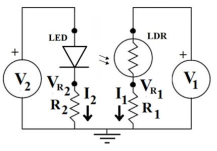
\includegraphics[width=.3\textwidth]{fig2}
  \caption{Esquemático montado para a segunda parte do experimento.}
  \label{fig:fig2}
\end{figure}

Os valores obtidos experimentalmente estão dispostos na tabela \ref{tab:q2}.


\begin{table}[H]
\centering
\caption{Comportamento do segundo circuito.}
\label{tab:q2}
\begin{tabular}{|c|c|c|c|c|c|c|}
\hline
$\mathbf{V_{R2 alvo}}$ & $\mathbf{V_{R2}}$ & $\mathbf{V_{R1}}$ & $\mathbf{I_{LED}}$ & $\mathbf{V_{LDR}}$ & $\mathbf{I_{LDR}}$ & $\mathbf{G_{LDR}}$ \\ \hline
\textbf{0.0}         & 0                 & 45.3m             & 0                  & $11.95 V$          & $0.44 m$           & $37.4\mu$          \\ \hline
\textbf{0.5}         & $0.500V$          & $0.985V$          & $0.5015 m$         & $11.01 V$          & $9.72 m$           & $882.7\mu$         \\ \hline
\textbf{1.0}         & $0.999V$          & $1.424V$          & $1.002m$           & $10.57 V$          & $14.05 m$          & $1.32m$            \\ \hline
\textbf{1.5}         & $1.501V$          & $1.725V$          & $1.505m$           & $10.27 V$          & $17.02 m$          & $1.65m$            \\ \hline
\textbf{2.0}         & $2.00V$           & $1.951V$          & $2.00m$            & $10.05 V$          & $19.25 m$          & $1.91m$            \\ \hline
\textbf{2.5}         & $2.50V$           & $2.14V$           & $2.507m$           & $9.86 V$           & $21.12 m$          & $2.15m$            \\ \hline
\textbf{3.0}         & $3.00V$           & $2.30V$           & $3.00m$            & $9.7 V$            & $22.70 m$          & $2.34m$            \\ \hline
\end{tabular}
\end{table}

As imagens para os resultados elencados podem ser verificados pelas medições vistas na figura \ref{fig:exp2_photos}.

\begin{figure}[H]
  \centering
  \begin{subfigure}{.3\textwidth}
    \centering
    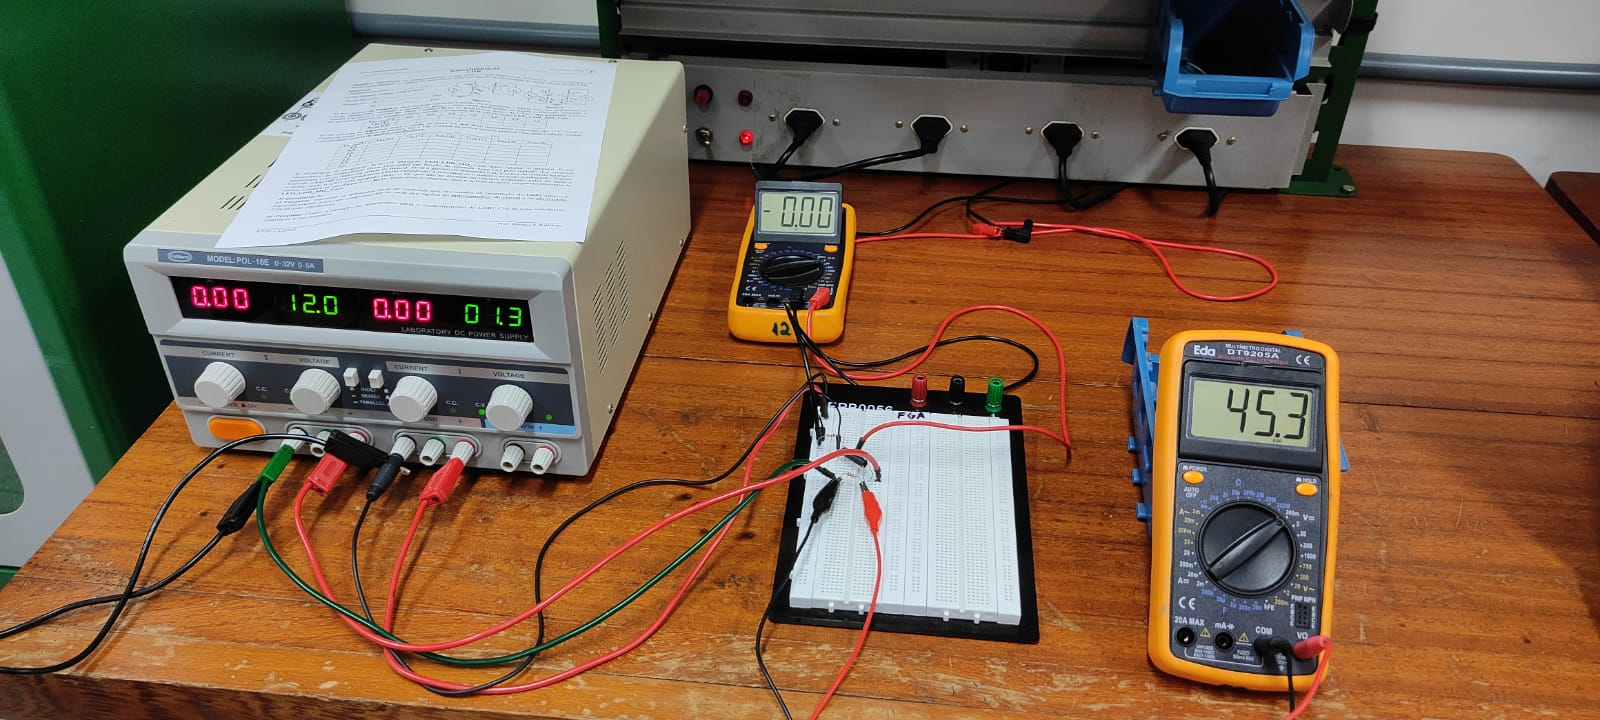
\includegraphics[width=\textwidth]{q2_0V}
    \caption{$VR2_{alvo}=0V$}
  \end{subfigure}
  \begin{subfigure}{.3\textwidth}
    \centering
    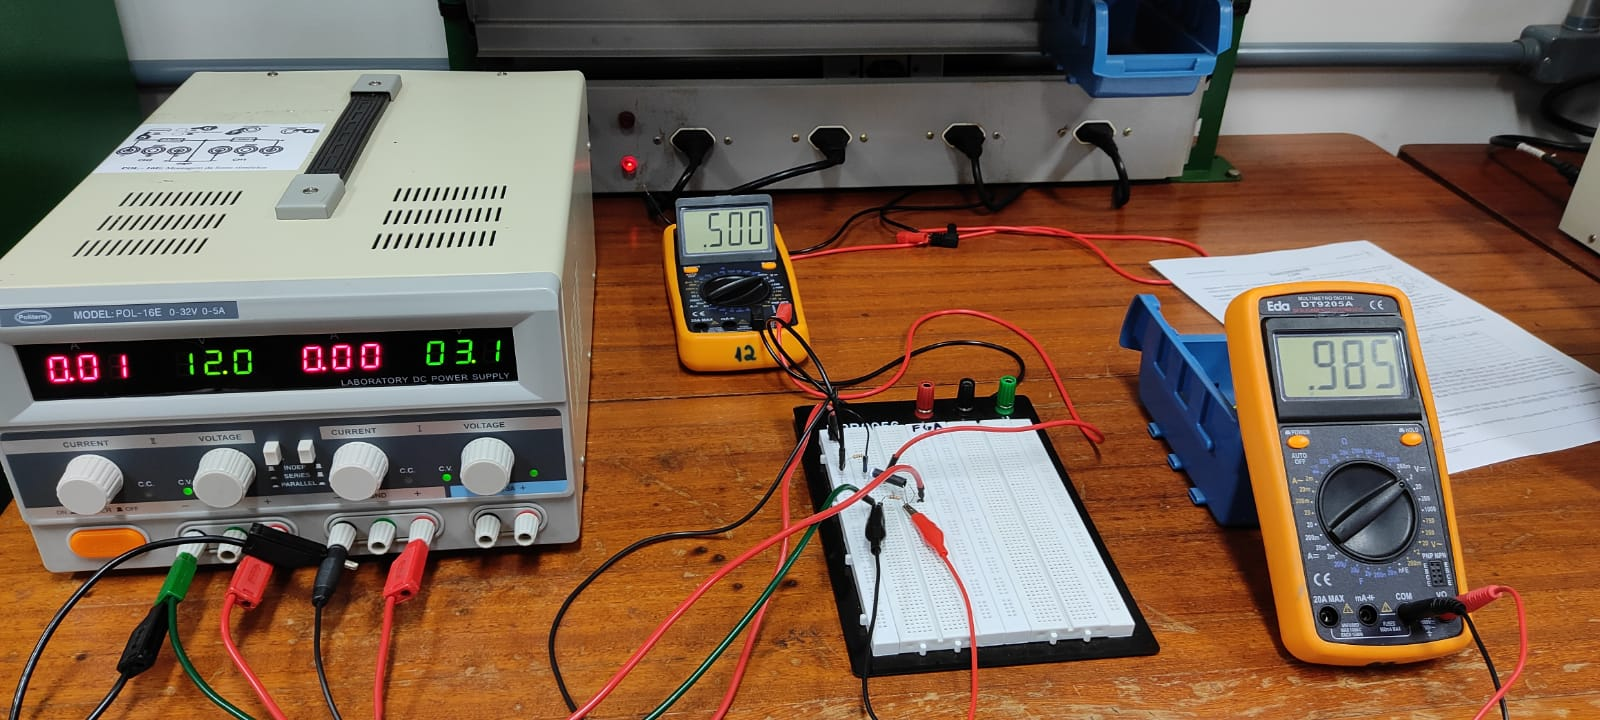
\includegraphics[width=\textwidth]{q2_0V5}
    \caption{$VR2_{alvo}=0.5V$}
  \end{subfigure}
  \begin{subfigure}{.3\textwidth}
    \centering
    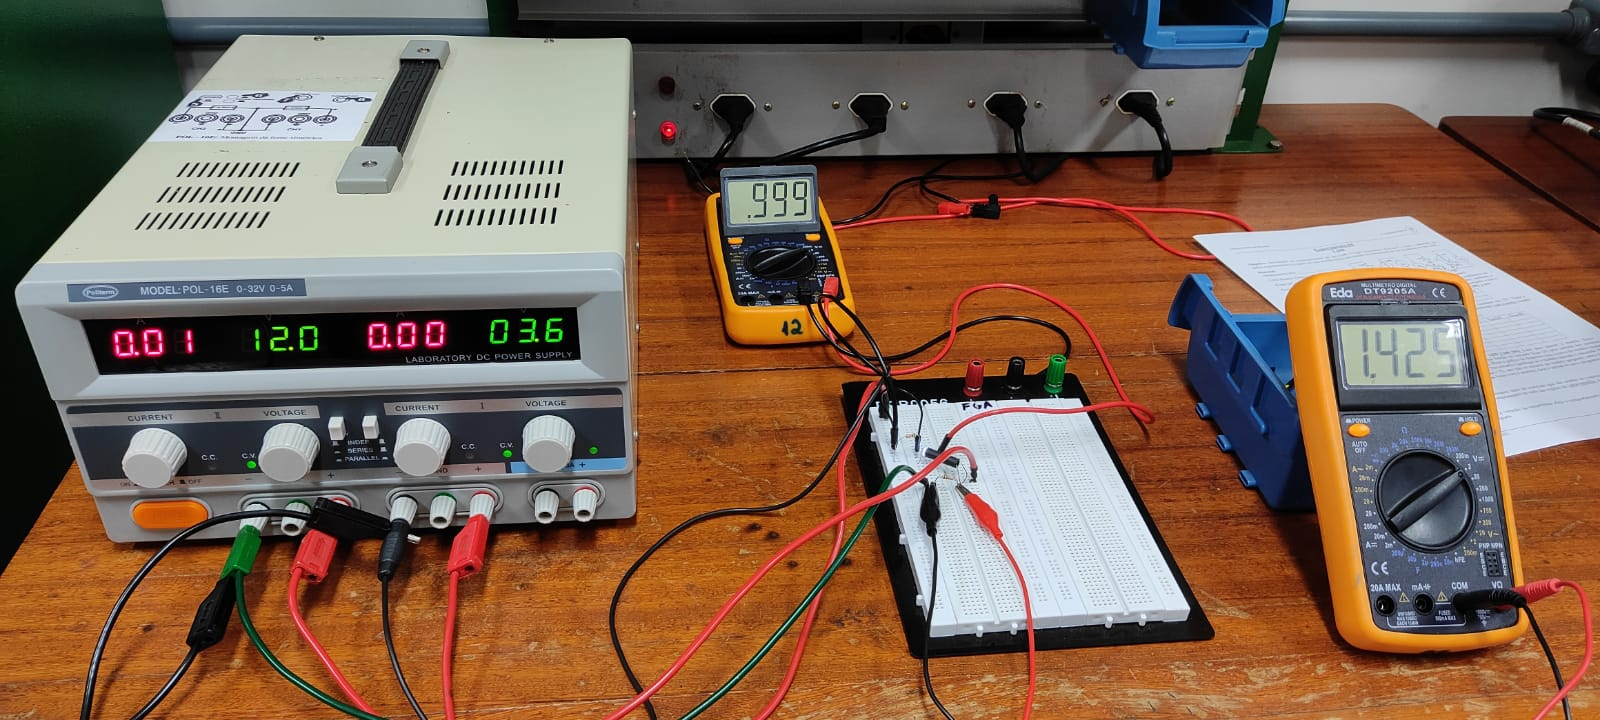
\includegraphics[width=\textwidth]{q2_1V}
    \caption{$VR2_{alvo}=1V$}
  \end{subfigure}
  \begin{subfigure}{.3\textwidth}
    \centering
    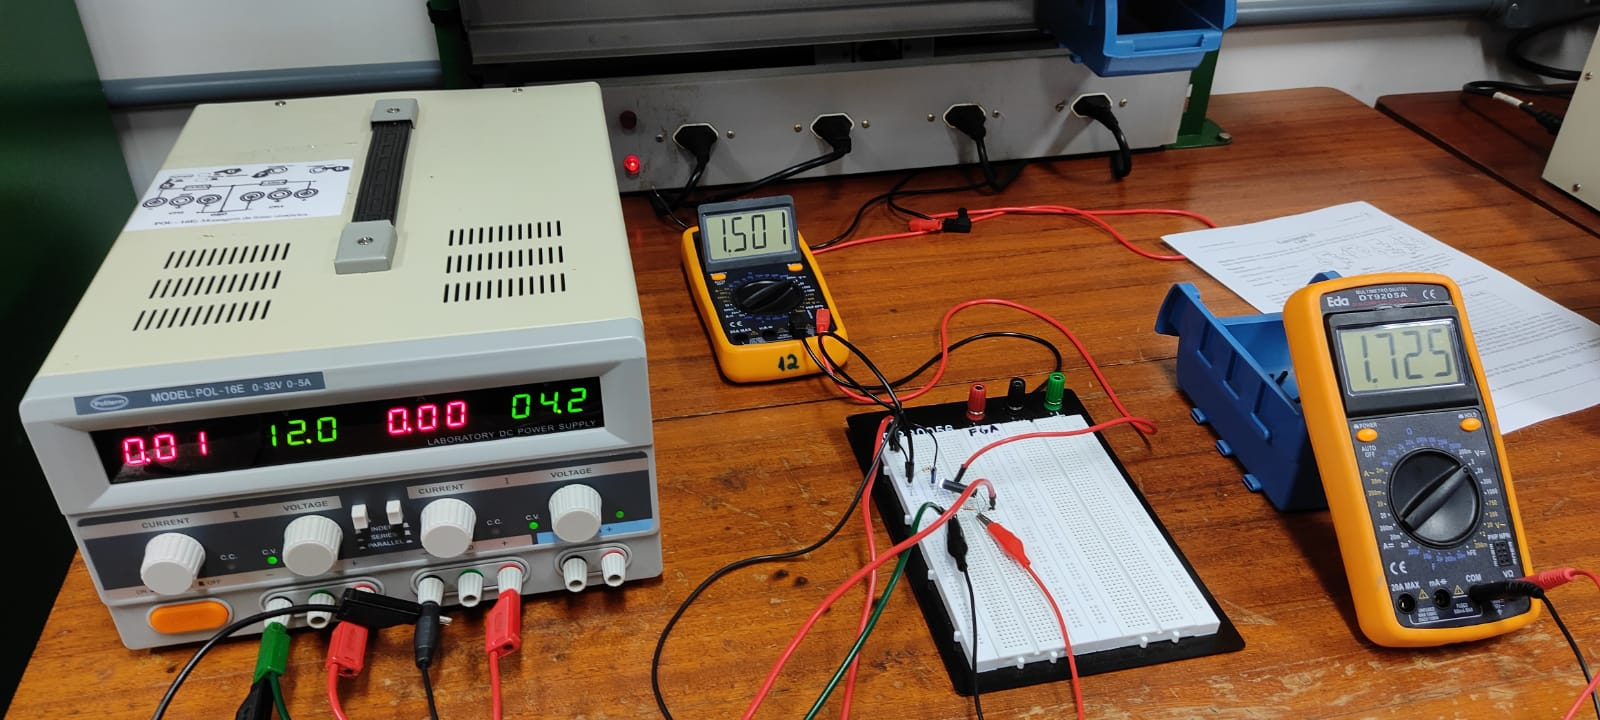
\includegraphics[width=\textwidth]{q2_1V5}
    \caption{$VR2_{alvo}=1.5V$}
  \end{subfigure}
  \begin{subfigure}{.3\textwidth}
    \centering
    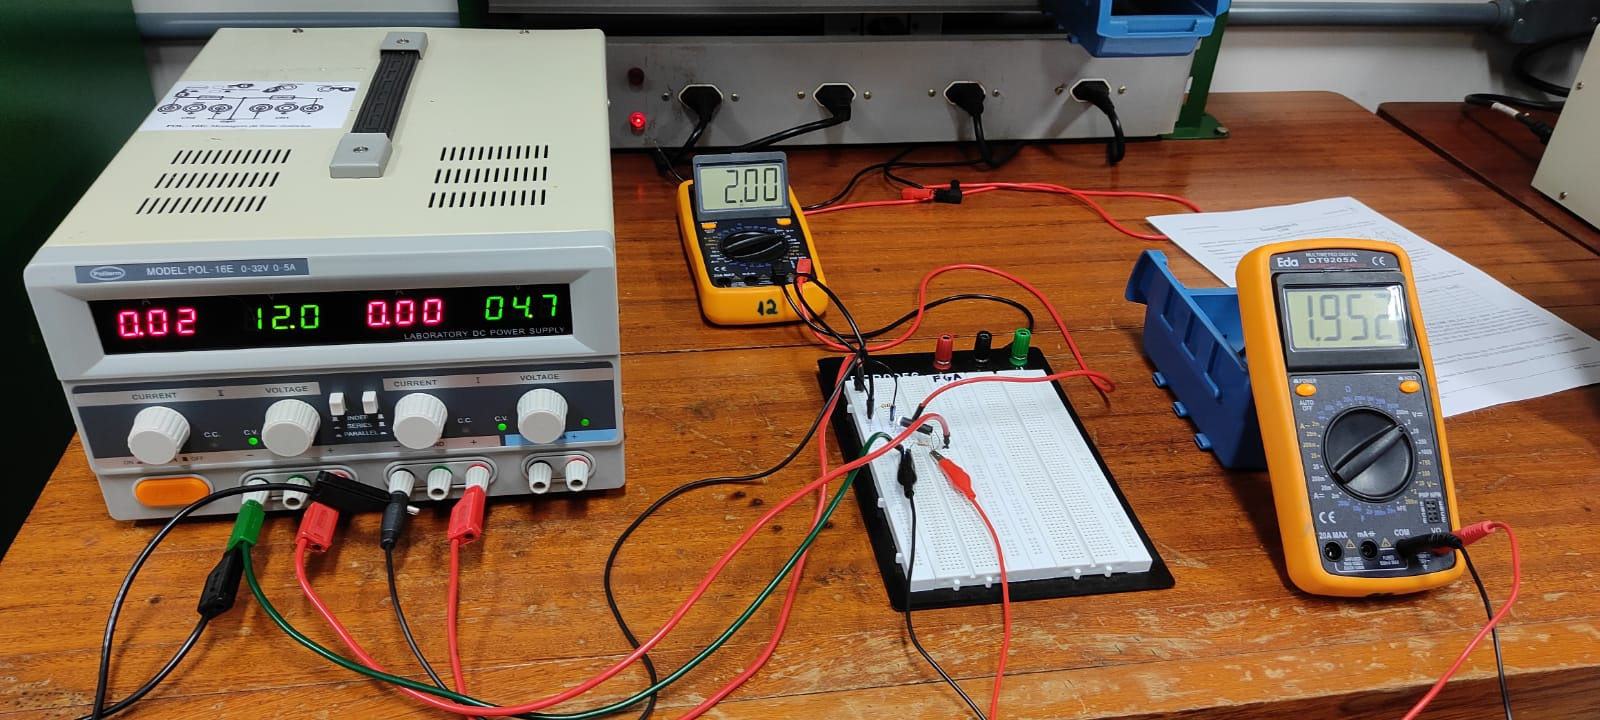
\includegraphics[width=\textwidth]{q2_2V}
    \caption{$VR2_{alvo}=2V$}
  \end{subfigure}
  \begin{subfigure}{.3\textwidth}
    \centering
    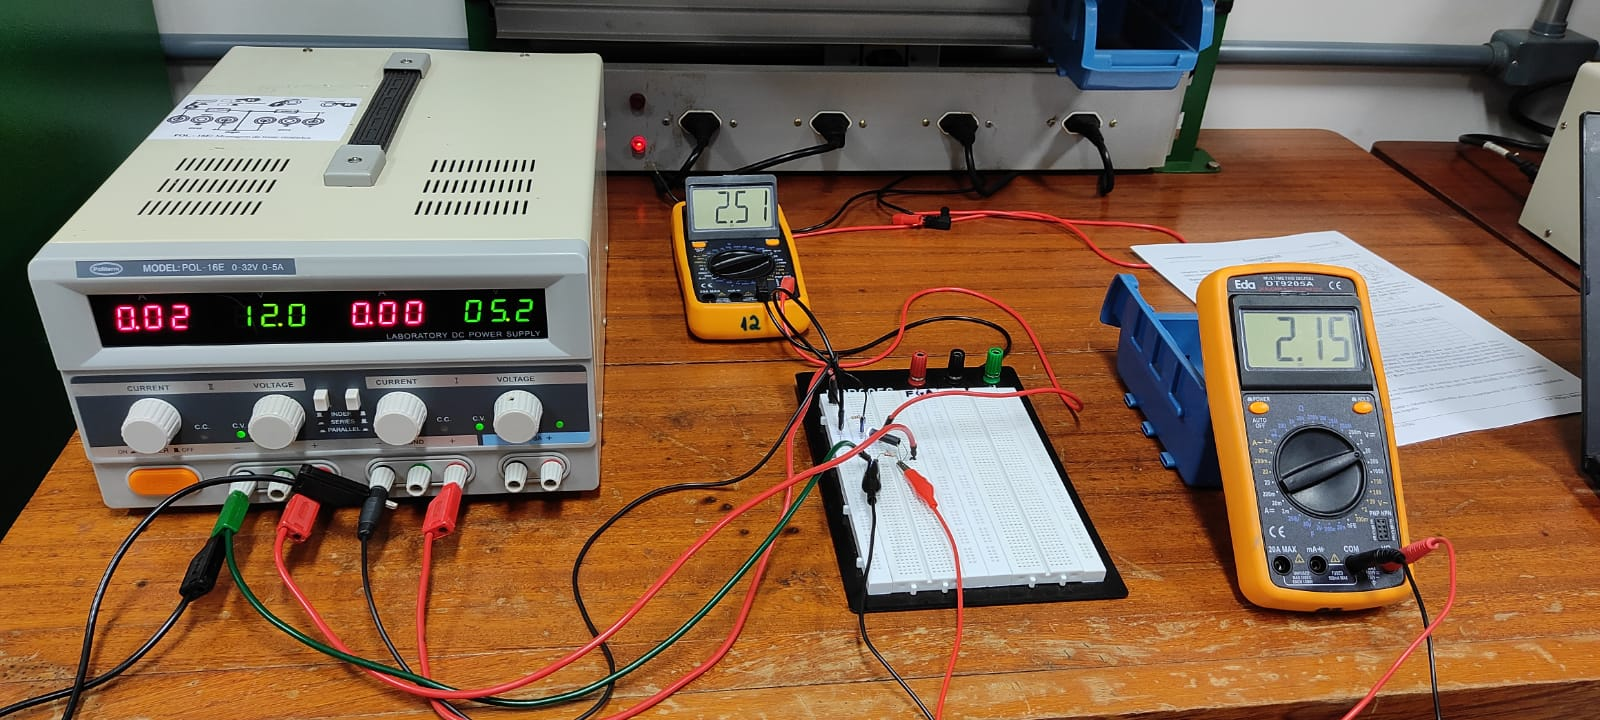
\includegraphics[width=\textwidth]{q2_2V5}
    \caption{$VR2_{alvo}=2.5V$}
  \end{subfigure}
  \begin{subfigure}{.3\textwidth}
    \centering
    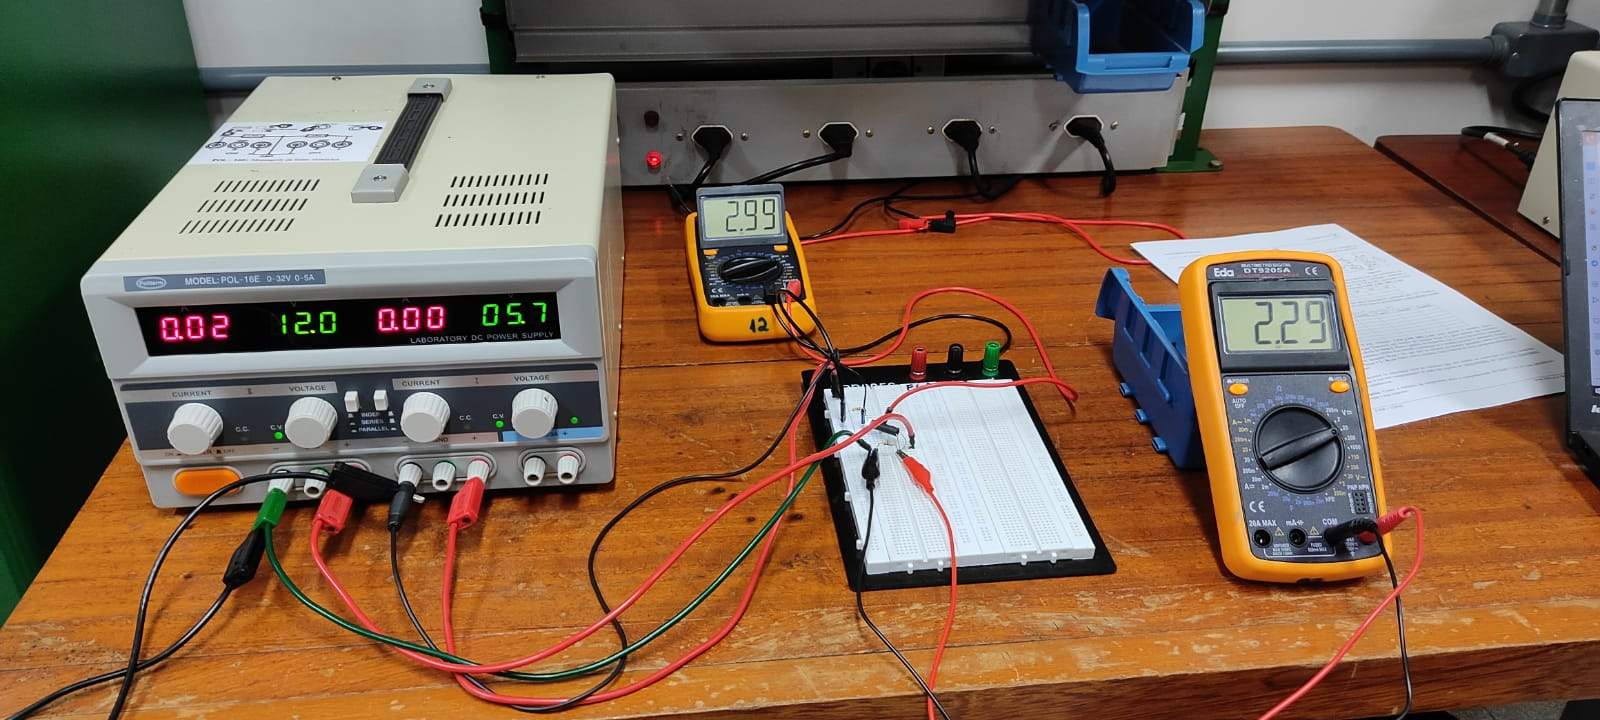
\includegraphics[width=\textwidth]{q2_3V}
    \caption{$VR2_{alvo}=3V$}
  \end{subfigure}
  
  \caption{Medições realizadas para a segunda parte do experimento.}
  \label{fig:exp2_photos}
\end{figure}




\subsection{Questão 3}

Tal gráfico já foi implementado na figura \ref{fig:q1_graph}. Em azul, tem-se o ajuste do modelo pelo método dos mínimos quadrados. 

\section{Questionário}


\subsection{Pesquisa: Encontre os diferentes tipos de materiais que são usados na construção de LDRs sensíveis especificamente à luz nos comprimentos de onda das regiões do infravermelho, do visível e do ultravioleta. Cite as suas referências.}

Na região do infravermelho próximo o mais utilizado é o sulfeto de chumbo (Pbs), enquanto no infravermelho médio usa se o antimoneto de índio (InSb). Na região do visível os mais utilizados são o sulfeto de cádimo (CdS) e o seleneto de cádimo (CdSe).

\textbf{Fonte: Rezende, Sergio Machado. Materiais e dispositivos eletrônicos. Editora Livraria da Física, 2004.}

\subsection{Pesquisa: Como a variação da temperatura afeta o comportamento do LDR? Cite as suas referências. Justifique a sua resposta.}

A temperatura representa uma certa quantidade de energia presente no dispositivo intrínsecamente. Assim, temos que como a temperatura representa o movimento das cargas, então tem-se que a temperatura é um gerador de ruído. O impacto disso na medição é que agora será necessário uma radiação mínima tal que seja maior que o ruído intrínseco, o que faz com que o limiar mínimo de detecção seja alterado e consequemtemente toda a curva característica do resistor LDR. 

\textbf{Fonte: Rezende, Sergio Machado. Materiais e dispositivos eletrônicos. Editora Livraria da Física, 2004.}

\section{Conclusão}

Com esse experimento, foi possível analisar completamente o comportamento dos resistores dependentes de luz. Como visto, eles apresentam uma impedância muito alta quando não estão expostos a luz, passando para uma resistência menor em várias ordens quando está exposto a algum tipo de luminosidade. Tal luminosidade não precisa ser tão alta, pois é possível realizar a medição de fontes de luz muito fracas, como o LED.

Dado isso, podemos aplicar esse dispositivos em diversos produtos, como é o caso do detector de luz solar, muito utilizado lâmpadas de postes, para o acendimento automático. Dependendo da sensibilidade do sensor, também pode ser utilizado em plantações artificiais, para controlar a taxa de luminosidade ideal sobre plantas, por exemplo.

\end{document}
